\documentclass[aps, twocolumn, floatfix, superscriptaddress]{revtex4}
\usepackage{amsmath, amssymb, amsfonts, gensymb}
\bibliographystyle{apsrev}
\usepackage{graphicx}
\graphicspath{ {Figures/} }
\newcommand{\tdc}[3][]{\frac{\mathrm{d}^{#1}#2}{\mathrm{d}#3^{#1}}} % total differential change.
\newcommand{\pdc}[3][]{\frac{\partial^{#1} #2}{\partial #3^{#1}}} % partial differential change.
\newcommand{\td}[1]{\mathrm{d}#1}
\newcommand{\pd}[1]{\partial#1}

\begin{document}

\title{Hydrodynamics of a Self-propelled C-boat}

\author{V. S. Akella}
\affiliation{Collective Interactions Unit, OIST Graduate University, 1919-1 Tancha, Onna-son, Okinawa, Japan 904-0495}
\author{D. K. Singh}
\affiliation{Collective Interactions Unit, OIST Graduate University, 1919-1 Tancha, Onna-son, Okinawa, Japan 904-0495}
\author{S. Mandre}
\affiliation{School of Engineering, Brown University, 182 Hope Street, Providence, RI 02906, USA}
\author{M. M. Bandi}
\affiliation{Collective Interactions Unit, OIST Graduate University, 1919-1 Tancha, Onna-son, Okinawa, Japan 904-0495}
\email[Corresponding Author: ]{bandi@oist.jp}

\date{\today}

\begin{abstract}
In the present work, we attempt to understand the dynamics of a \emph{c-boat} at the air-water interface. A \emph{c-boat} is a disc-shaped agarose gel tablet with all the water in the agarose gel replaced by camphoric acid. Camphoric acid spreads over the air-water interface due to the interfacial tension forces creating concentration gradients which in turn cause the interfacial tension gradients around the c-boat. The asymmetry in the interfacial tension gradients spontaneously set the c-boat in motion at the air-water interface. Furthermore, we observe three different modes of motion, namely continuous, harmonic and periodic, due to the evaporation/sublimation of camphoric acid. We explain these modes in terms of ratio of two time scales, $\tau_{\eta}$ and $\tau_{\sigma}$, where $\tau_{\eta}$ is the time required for the development of Marangoni forces to overcome the viscous forces and $\tau_{\sigma}$ is the time during which Marangoni forces dominate the viscous forces. The continuous, harmonic and periodic motions are observed when $\frac{\tau_{\eta}}{\tau_{\sigma}} \approx 1$,  $\frac{\tau_{\eta}}{\tau_{\sigma}} >~ 1$ and $\frac{\tau_{\eta}}{\tau_{\sigma}} >> 1$ respectively. Experimentally, the ratio of the time scales is varied by changing the interfacial tension of the air-water interface using Sodium Dodecyl Sulfate (SDS).
\end{abstract}

\maketitle
\section{Introduction}
\section{Experimental Section}
\subsection{Materials and Methods}
\label{sec:prep}
A \emph{c-boat} is a disc-shaped agarose gel tablet, with all the water in the agaorse gel matrix replaced with camphoric acid. The identical nature of c-boats is of crucial importance if one wishes to characterize/study a collection of c-boats. Note that, all the experiments in this research work are carried out with c-boats of $3\ \mathrm{mm}$ diameter and $1\ \mathrm{mm}$ thickness. The preparation of the c-boats involves the following steps. 
\begin{enumerate}
\item Preparation of 5\% w/v agarose (Wako Pure Chemical Industries, Ltd., Cat. No. 346-00072) gel sheets of uniform thickness.
\item Punching out (using Biopunch, Ted Pella, Inc.) discs of agarose gel of required disc diameter. 
\item Soaking the agarose discs in camphoric acid (Wako Pure Chemical Industries, Ltd., Cat. No. 036-01002) saturated methanol (Wako Pure Chemical Industries, Ltd., Cat. No. 138-01836) solution for more than 2 hrs. This process replaces the water from the agarose gel with camphoric acid saturated methanol solution. 
\item Washing and rinsing of the discs in de-ionized water (obtained from Milli-Q Integral Water Purification System with resistivity, $\rho=\mathrm{18\ M} \Omega\ \mathrm{cm}$ at 25 $\celsius$). This step results in (1) the evaporation of methanol and (2) the precipitation of camphoric acid in the agarose gel matrix.
\end{enumerate}
When needed, we used Sodium Dodecyl Sulfate (Wako Pure Chemical Industries, Ltd., Cat. No. 196-08675) to modify the air-water interfacial tension.
\label{sec:expset}
\begin{figure}[ht]
    \begin{center}
       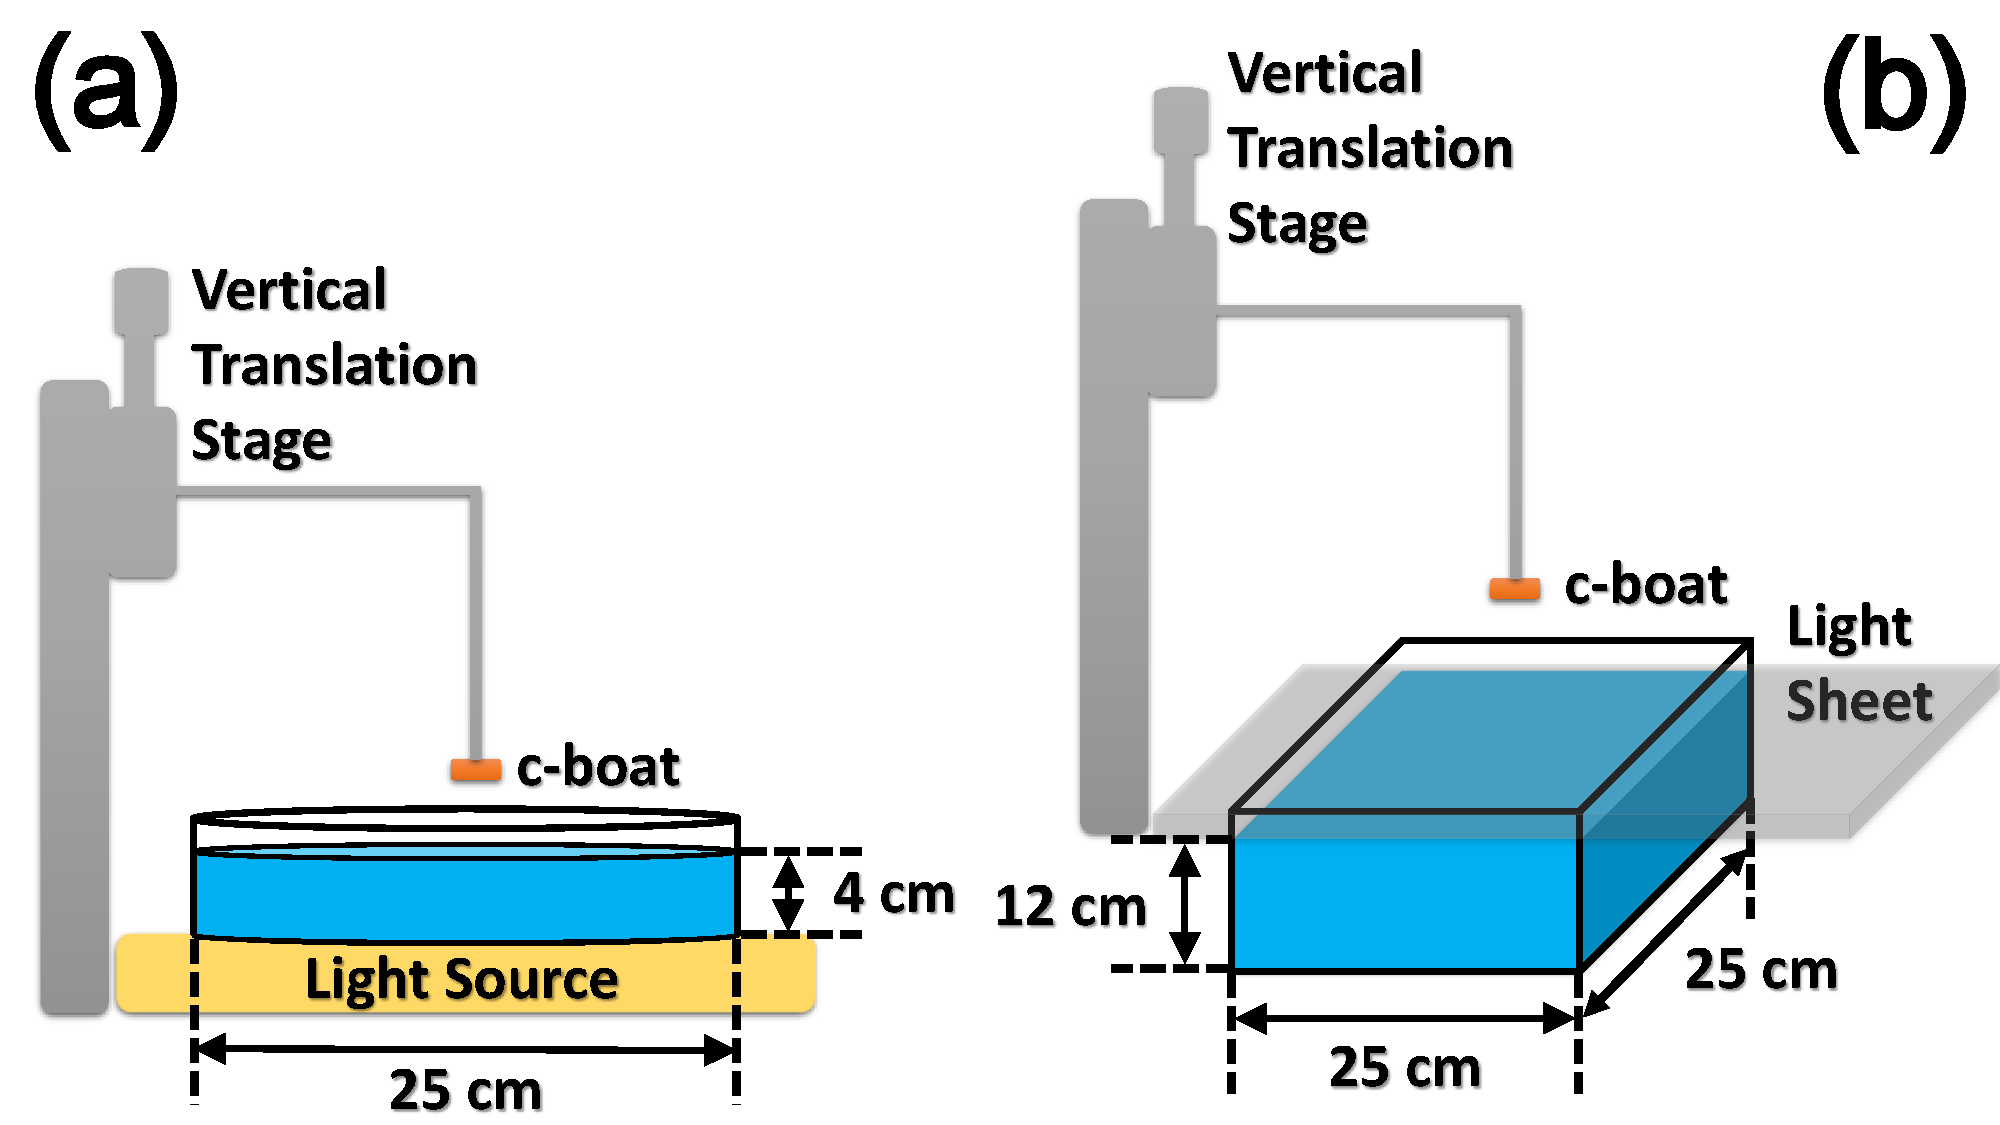
\includegraphics[scale=0.25]{figure1.pdf}
    \end{center}
    \caption{Experimental Setup.}
    \label{fig:expset}
\end{figure}
\subsection{Data Acquisition and Analysis}
The experimental setup (figure~\ref{fig:expset}) consists of (1) a glass container filled with de-ionized water (2) an L-shaped steel wire with one end firmly attached to a vertical translation stage (3) an illumination source and (4) Phantom v641 hi-speed camera, located directly above the glass container. The c-boat is attached at the free-end of the steel wire. At the beginning of the experiment the steel-wire-arrangement is lowered using the tranlational stage such that the c-boat gently makes a contact with the air-water interface and for the rest of the experiment the c-boat is left un-disturbed. For the transient regime experiments (figure~\ref{fig:expset}a), we used a 25 $\mathrm{cm}$ diameter and 5 $\mathrm{cm}$ height glass petri dish filled with approximately 2 liters of de-ionized water and the petri dish is illuminated using a light tablet from bottom. To visualize the spread dynamics, the air-water interface is covered with hydrophilic tracer particles ($d = 50\ \mu \mathrm{m}$, specific gravity = 0.25) at low packing fractions, $\phi \leq 0.2$. We did \emph{not} observe any effect of tracer particles on the spread dynamics at packing fractions, $\phi \leq 0.2$. The spread dynmics are recorded at 1000 frames per second with 100 $\mu \mathrm{s}$ exposure time using the hi-speed camera. As the camphoric acid spreads over the interface, the tracer particles are pushed away radially outwards creating a particle-free zone. The radius of the particle-free zone is measured manually from a time series of images (using ImageJ). Figure~\ref{fig:cspreadimg} shows the particle-free zone at an instant in time. For the steady state regime experiments (figure~\ref{fig:expset}b), we used a glass container of dimensions 25 $\mathrm{cm}$ $\times$ 25 $\mathrm{cm}$ $\times$ 25 $\mathrm{cm}$ filled with approximately 8 liters of de-ionized water and the air-water interface is illuminated with a laser sheet of thickness $\approx$ 3 $\mathrm{mm}$ such that the bulk layers are minimally illuminated. The fluid velocity at the interface is measured by mixing un-measurably small quantity of neutrally buoyant tracer particles ($d < 10\ \mu \mathrm{m}$). The motion of the tracer particles is recorded at 300 frames per second with 1 $\mathrm{ms}$ exposure time using the hi-speed camera. Figure~\ref{fig:radvelimg} is a resultant image obtained by adding 30 consecutive frames. The lengths of the streaks are manually measured (using ImageJ). The length of the streak, $\td{r}$ (figure~\ref{fig:radvelimg}) is the distance in centimeters (converted to centimeters using appropriate pixel to centimeter conversion factor) traveled by the tracer particle in $\td{t}=$ 0.1 $\mathrm{sec}$ at a radial distance $r$ (figure~\ref{fig:radvelimg}) from the center of the c-boat. 

\begin{figure}[ht]
\centering
  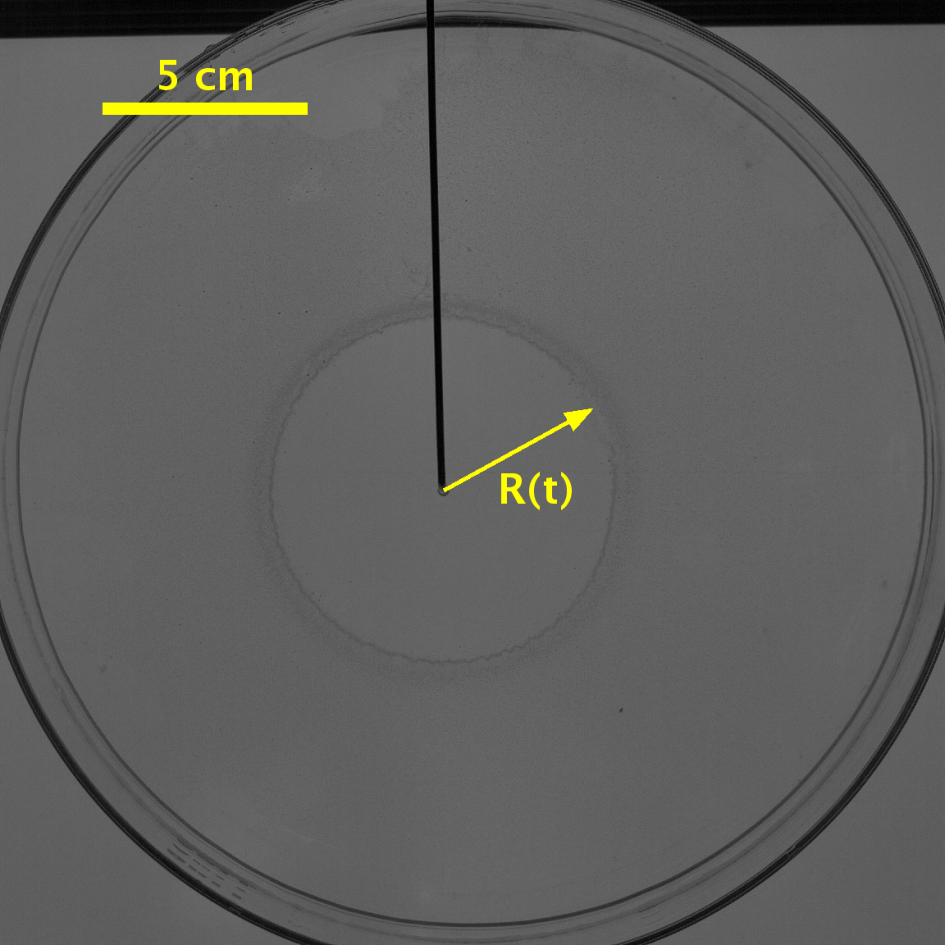
\includegraphics[width=0.8\columnwidth]{figure2.pdf}
  \caption{Caphoric acid spread radius at an instant in time, visualized using hydrophilic tracer particles.}
  \label{fig:cspreadimg}
\end{figure}
\begin{figure}[ht]
  \centering
  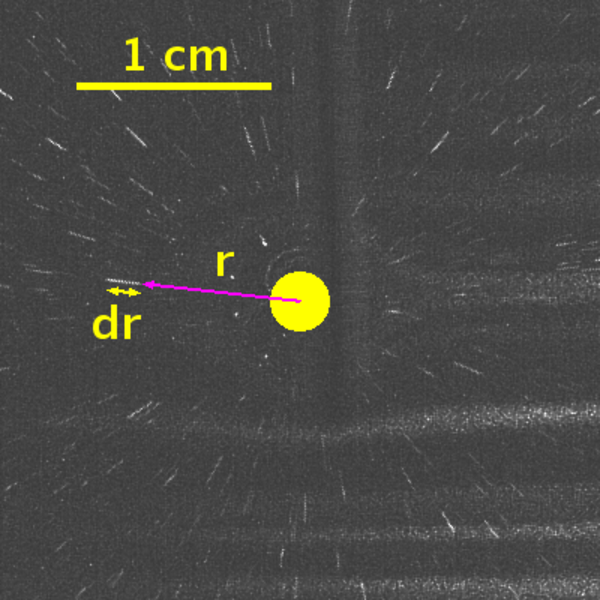
\includegraphics[width=0.8\columnwidth]{figure3.pdf}
  \caption{Measurement of radial velocity at a distance $r$ from the center of the c-boat. The length of the streak, $\td{r}$ is the distance traveled by the tracer particle in time $\td{t} = 0.1\ \mathrm{sec}$}
       \label{fig:radvelimg}
\end{figure} 

\section{Results and Discussion}
When a c-boat is placed at the air-water interface, camphoric acid is drawn out of the c-boat by the interfacial tension forces to minimize the interfacial free energy and the camphoric acid front emanates radially outwards. Due to the evaporation/sublimation of camphoric acid, the spreading can \emph{not} continue until interface is saturated with the camphoric acid. Owing to the slower evaporation/sublimation kinetics of camphoric acid compared to the spread dynamics, the concentration front spreads to a farther distance than \emph{the steady state distance}. The \emph{steady state distance} is defined as the distance, measured from the center of the c-boat, at which the advection flux and the evaporation flux of camphoric acid balance each other. As a result, the concetration front retraces to the steady state distance (see movie S1 in the supplementary information). Note that, the hydrophilic tracer particles trace back because by spreading they minimize the interfacial energy of air-water interface. For brevity, we discuss our findings in two parts, 1. The transient regime and 2. The steady state regime. 
\subsection{Transient Regime}
\label{sec:transient}
The transient regime is observed from the instance of c-boat's contact with the air-water interface to the time when the camphoric acid spread radius reaches a steady state value. During the transient regime, we observe two spreading stages (1) the divergent stage: during which the camphoric acid molecules are drawn out of the c-boat and spread radially outwards over the interface soon after the c-boat's contact with the air-water interface (2) the convergent stage: during which the spread radius shrinks to the steady state value due to evaporation/sublimation of camphoric acid. The spread radius, measured during the divergent stage, follows a power law in time with a scaling exponent of $t^{1/2}$ which is in agreement with the observed scaling for the spread of volatile oils at the air-water interface (ref). Note that, this is \emph{not} the observed scaling with non-volatile oils, for which the spread radius scales with time as $t^{3/4}$ (ref). Figure~\ref{fig:caspread} is a plot of the spread radius $R(t)$ as a function of time measured during divergent stage. We attribute the scatter in the data around the fit to the experimental variation in the depth of c-boat sitting below the air-water interface.   

\begin{figure}[ht]
    \begin{center}
       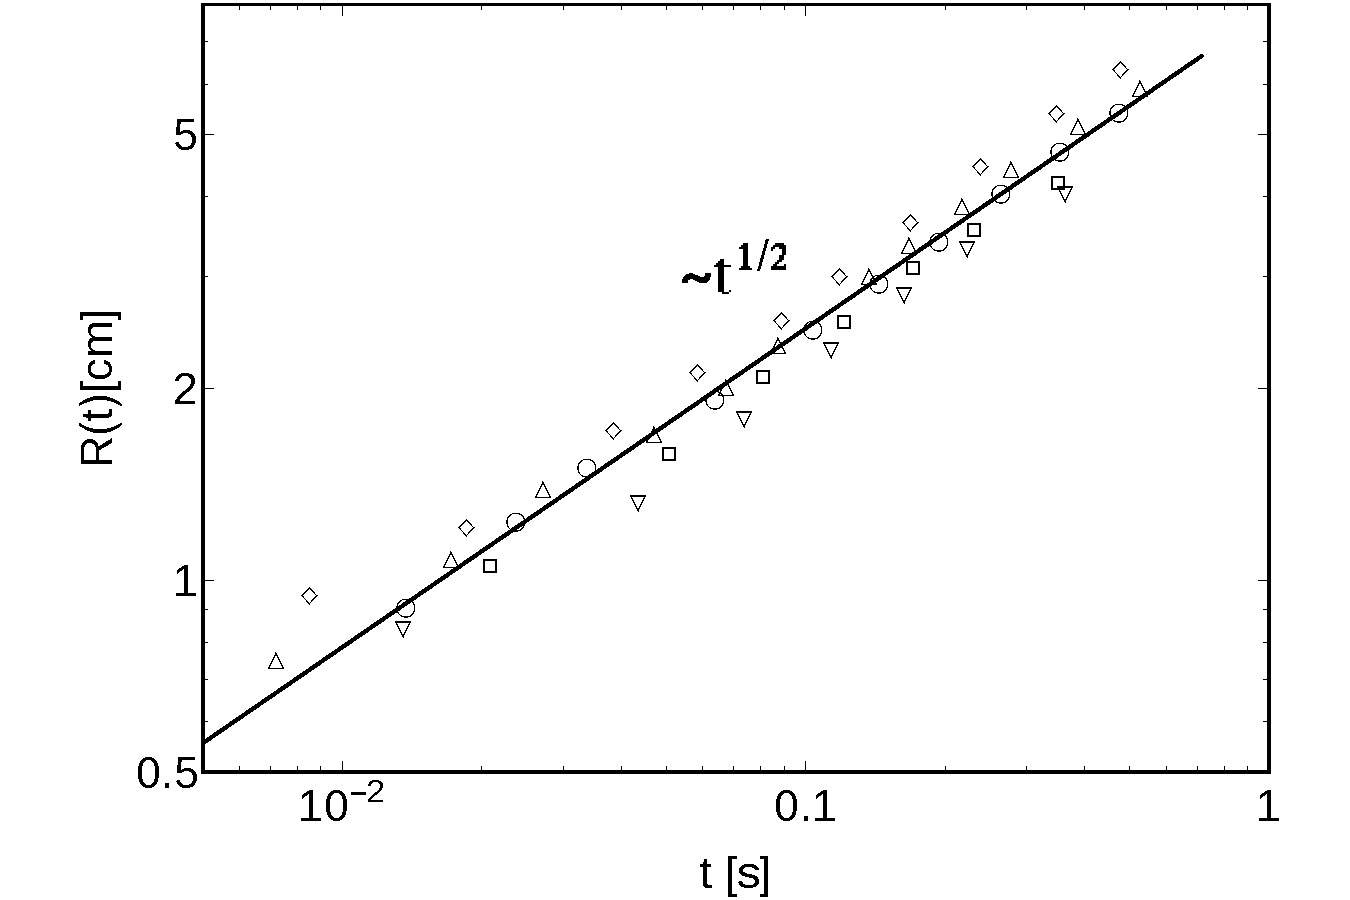
\includegraphics[scale=0.35]{figure4.pdf}
    \end{center}
    \caption{Camphoric acid radial spread vs. time. The radial front is visualized using 50 $\mu m$ hydrophilic tracer particles sparsely sprinkled at the air-water interface. }
    \label{fig:caspread}
\end{figure}

\subsection{Steady State Regime}
\label{sec:steady}
The spread of camphoric acid over the air-water interface reaches a steady state when the advection flux equals the evaporation flux. The radial distance, measured from the center of c-boat, at which the flux balance is achieved happens to be smaller than the maximum spread distance measured in the divergent stage (explained in section~\ref{sec:transient}) because of slower evaporation/sublimation kinetics than the spread dynamics. Note that, camphoric acid poorly dissolves in water and the amount of camphor entering the bulk water is negligible. However, the camphoric acid adsorbed at the air-water interface is sufficient enough to change the interfacial tension of air-water interface. As a result camphoric acid concentration gradients are setup around the c-boat. These concetrations gradients lead to the interfacial tension gradients and are the source of solutal Marangoni forces. When there is no evaporation, the spread dynamics \emph{never} reach a steady state. Note that, in a finite-sized system the spread dynamics reach a steady state when the air-water interface is saturated with the non-volatile oil. However, there will \emph{not} be concetration gradients to drive fluid flow are \emph{never} setup since there is no evaporation. Therefore, evaporation is a very critical requirement in our analysis. The Marangoni froces shear the air-water interface and cause the underlying fluid flow. The fluid flow penetrate into bulk due to the viscosity of the bluk fluid. We derive a scaling law for the radial velocity of the fluid flow at the air-water interface using boundary layer approximation. Let $c(r)$ and $v(r)$ be the concentration and velocity profiles at the air-water interface. Then the flux of camphor $q$ at a radial distance $r$ is: 
\begin{equation}
q \approx r u_{r} c \implies c \approx \frac{q}{ru_{r}} 
\end{equation}
Order of magnitude estimation yields:
\begin{equation}
C = \frac{Q}{RU_{r}}
\end{equation}
Assuming that intefacial tension $\sigma (r)$ varies linearly with concentration $c(r)$. The solutal Marangoni force is:
\begin{equation}
\sigma (r) = -k c(r) + \sigma_{0} \implies \tdc{\sigma}{r} = -k\tdc{c}{r}  \approx k \frac{C}{R}
\end{equation}
where, $k$ is the rate of evaporation/sublimation. 
Boundary layer approximation and continuity equation yield: 
\begin{align}
u_{r}\pdc{u_{r}}{r} + u_{z}\pdc{u_{r}}{z} &= \nu \pdc[2]{u_{r}}{z} \\
\pdc{(ru_{r})}{r} + r\pdc{u_{z}}{z} &= 0
\end{align}
Order of magnitude calculations yield:
\begin{align}
\frac{U_{r}^{2}}{R} \approx \frac{U_{r}U_{z}}{\delta} &\approx \frac{\nu U_{r}}{\delta^{2}} \\ 
\frac{U_{r}}{R} &\approx \frac{U_{z}}{\delta} 
\end{align}
Simplifying above equations yield:
\begin{equation}
\delta = \sqrt{\frac{\nu R}{U_{r}}}
\end{equation}
At the air-water interface, the Marangoni stresses are balanced by the viscous stresses. Mathematically,
\begin{equation}
k\tdc{c}{r} = \mu \tdc{u_{r}}{z} \implies \frac{kC}{R} = \frac{\mu U_{r}}{\delta}
\end{equation}
Substituting equations (??) and (??) 
\begin{equation}
\frac{kQ}{U_{r}R^{2}} = \frac{\mu U_{r}}{\sqrt{\frac{\nu R}{U_{r}}}} \implies
\boxed{U_{r} = \left(\frac{kQ\nu^{1/2}}{\mu}\right)^{2/5} R^{-3/5}}
\end{equation}
\begin{figure}[ht] 
    \begin{center}
       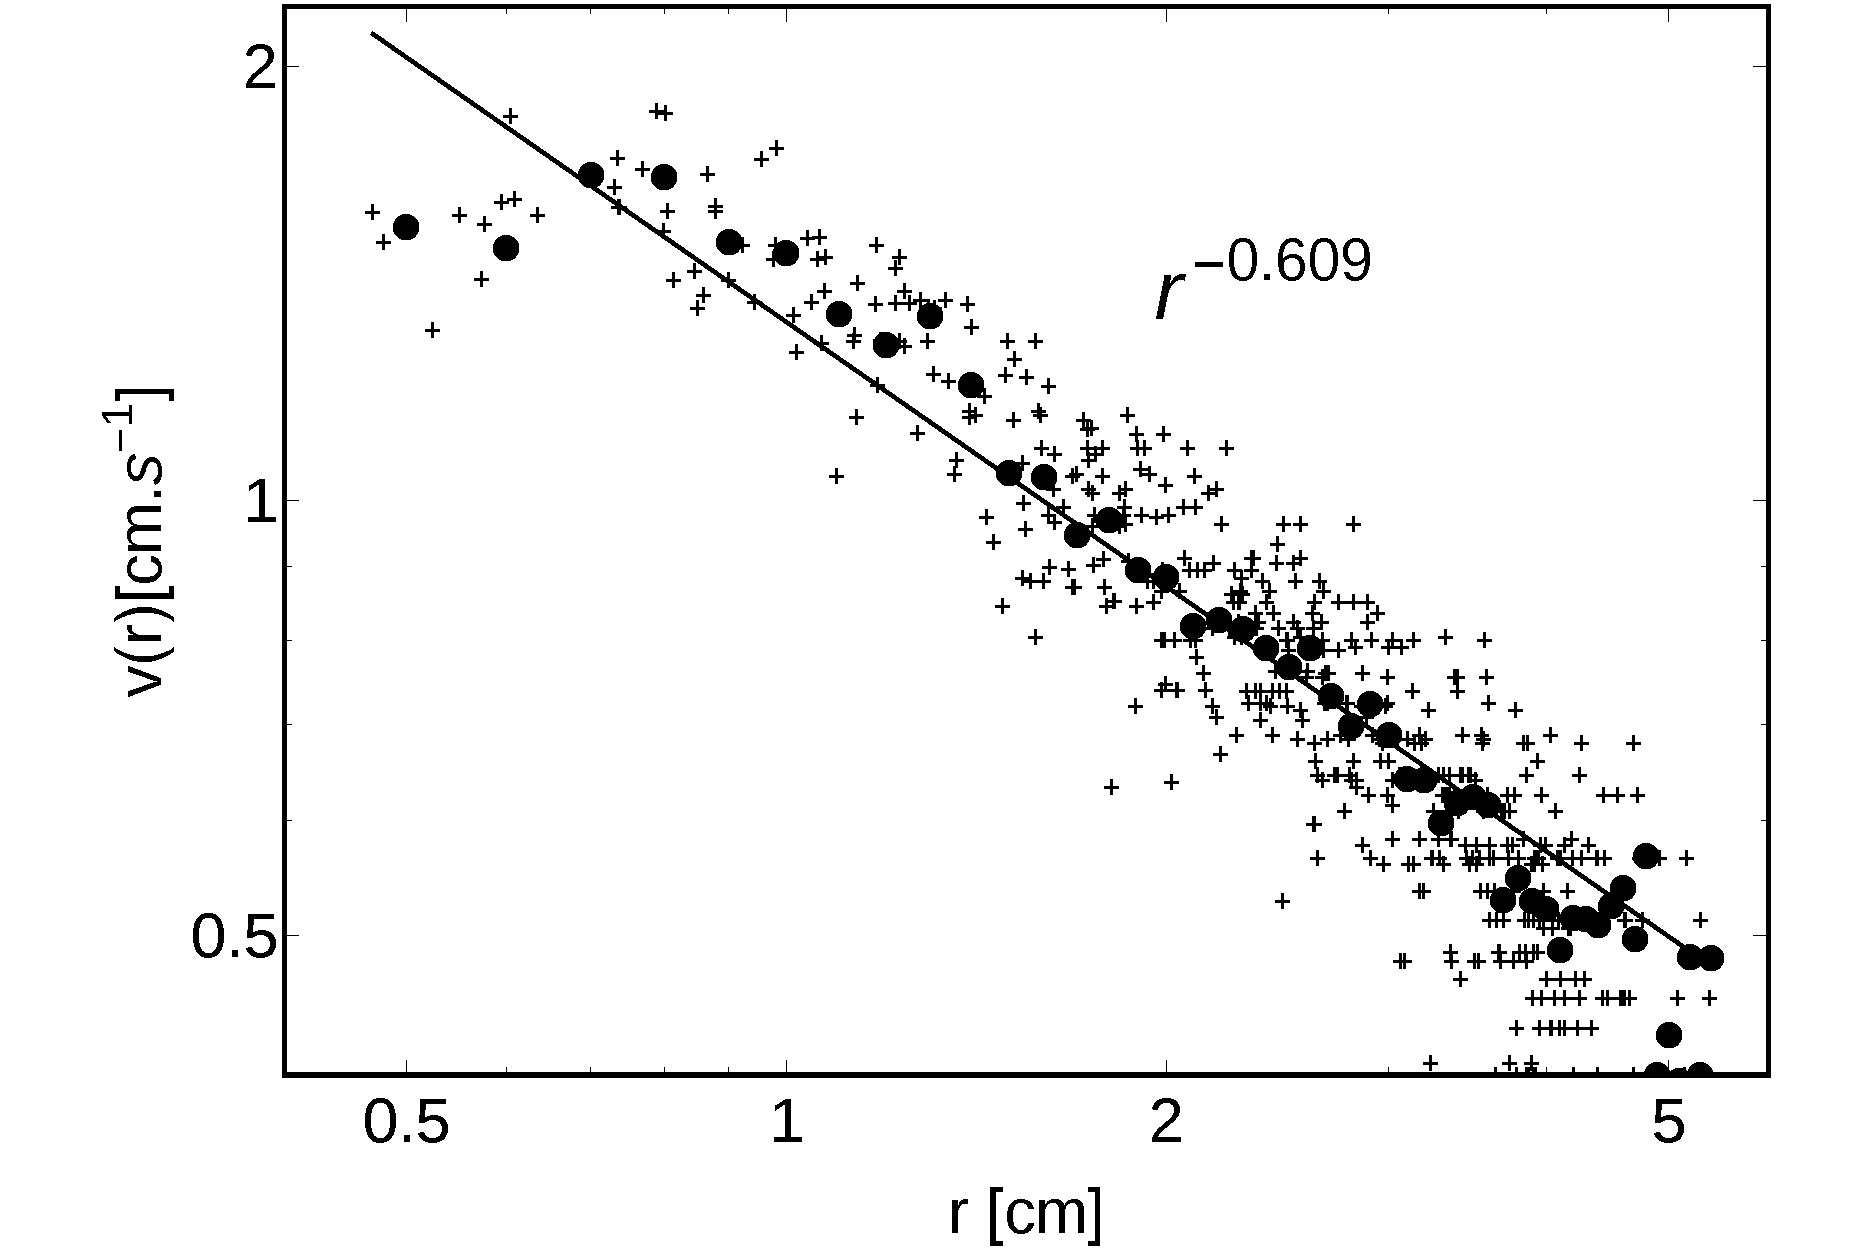
\includegraphics[scale=0.25]{figure5.pdf}
    \end{center}
    \caption{Radial velocity measured at the air-water interface}
    \label{fig:radvel}
\end{figure}
\section{Dynamic C-boat}
When the c-boat is placed at the air-water interface, the following processes lead to the movement of c-boat on the air-water interface.
\begin{itemize}
\item Camphoric acid spreads onto the air-water interface via two processes. 1. Interfacial forces draw the camphoric acid molecules out of the c-boat to minimize the interfacial energy. 2. Diffusion of camphoric acid molecules onto the air-water interface. Dissolution is another mechanism by which camphoric acid is drawn out of c-boat but it is very minimal as the solubility of camphoric acid is $\approx$ 40 mM at 25 \celsius.
\item As mentioned earlier, camphoric acid is a surface active molecule and lowers the air-water interfacial energy. When a c-boat is introduced at the air-water interface, the out-flux of camphoric acid molecules from the c-boat sets up interfacial tension gradients symmetrically around the c-boat. A random perturbation arising due to change in local temperature or contamination of air-water interface due to unavoidable dust particles in air spontaneously break the symmetric interfacial tension gradients around the c-boat. When the perturbation is strong enough to overcome the viscous drag forces on the c-boat, the c-boat starts moving. Once the c-boat starts moving it further enhances the asymmetry resulting in continuous motion of the c-boat.
\item The air-water interface never gets saturated with the camphoric acid because camphoric acid sublimes into room. Therefore the motion of the c-boat lasts as long as there is camphoric acid in the c-boat.
\end{itemize}
\subsection{Lifetime of a C-boat}
\label{sec:lifetime}
The forces acting on the c-boat are, 1. Marangoni forces set up by the interfacial tension gradients which are in turn caused camphoric acid concentration gradients, 2. Drag forces due to the viscosity of the medium. During the course of the experiment, camphoric acid sublimes into the surroundings resulting in decrease in Marangoni forces. Another mechanism that affects the lifetime of a c-boat is: the dissolution of camphoric acid in water which decreases the background air-water interfacial tension resulting in lesser interfacial tension gradients. However, the amount of camphoric acid in a c-boat ($\simeq 7\ \mathrm{mg}$) is negligibly small to modify the interfacial tension of water by a measurable amount. The interfacial tension of water, when saturated with camphoric acid ($\simeq 8\ \mathrm{g/l}$), is $\simeq 60\ \mathrm{dy/cm}$. As camphoric acid sublimes the physical characteristics of the system change continuously. Figure~\ref{fig:lifetime} is the speed of a c-boat as function of time. 
\begin{figure}[ht]
    \begin{center}
       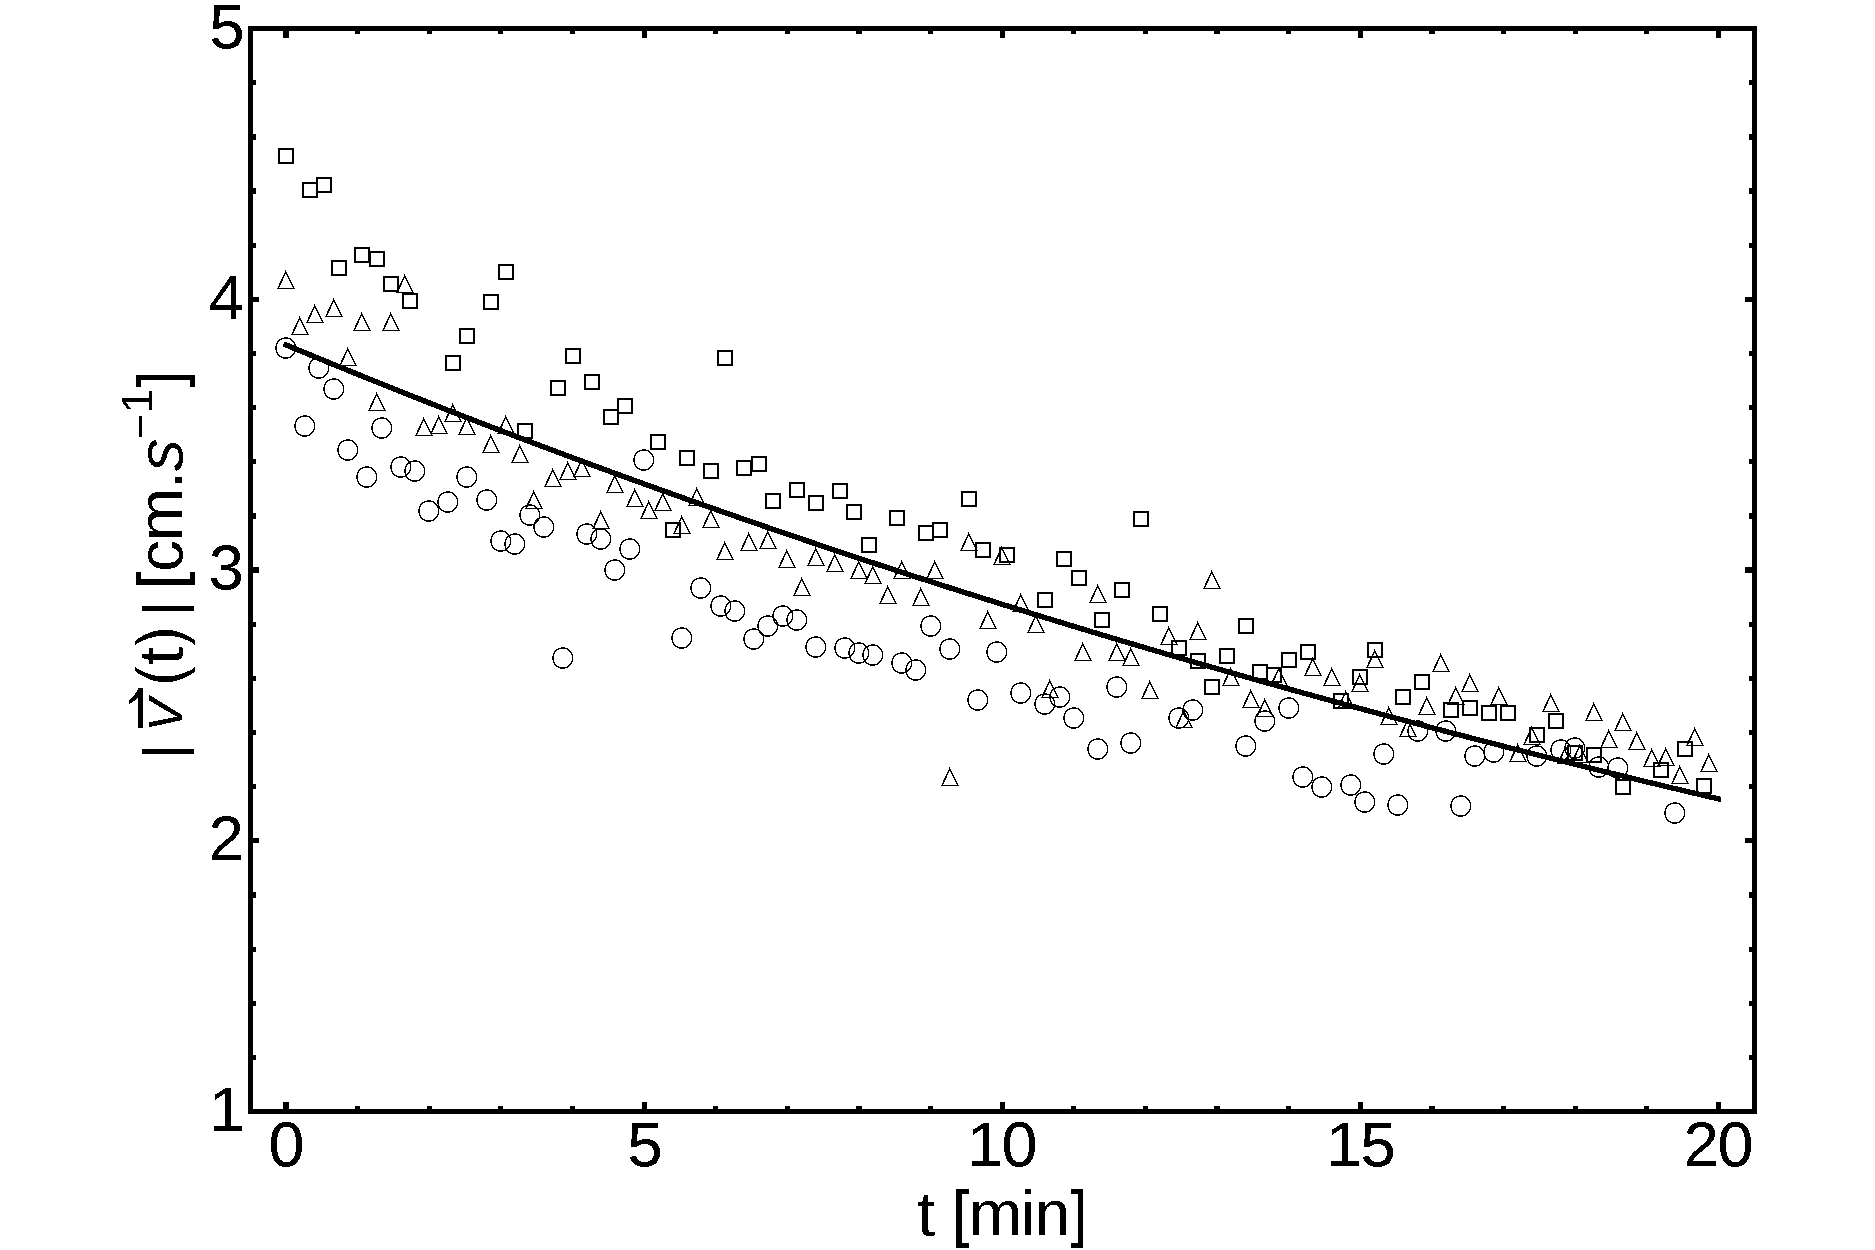
\includegraphics[scale=0.25]{figure6.pdf}
    \end{center}
    \caption{Lifetime of the c-boat.}
    \label{fig:lifetime}
\end{figure}
\subsection{Oscillatory Motion of the C-boat}
\label{sec:movingc-boat}
Another interesting phenomenon observed in c-boat dynamics is the oscillatory motion of the c-boat. Figure~\ref{fig:absvnosds} shows the time traces of the c-boat speed at different intervals and the corresponding power spectra. At the beginning of the experiment there is a strong peak at $\approx 1\ \mathrm{Hz}$ in the power spectrum. However the peak completely disappears at long times. The observed phenomenon is shown in figure~\ref{fig:absvnosds}.   
\begin{figure}[ht]
    \begin{center}
       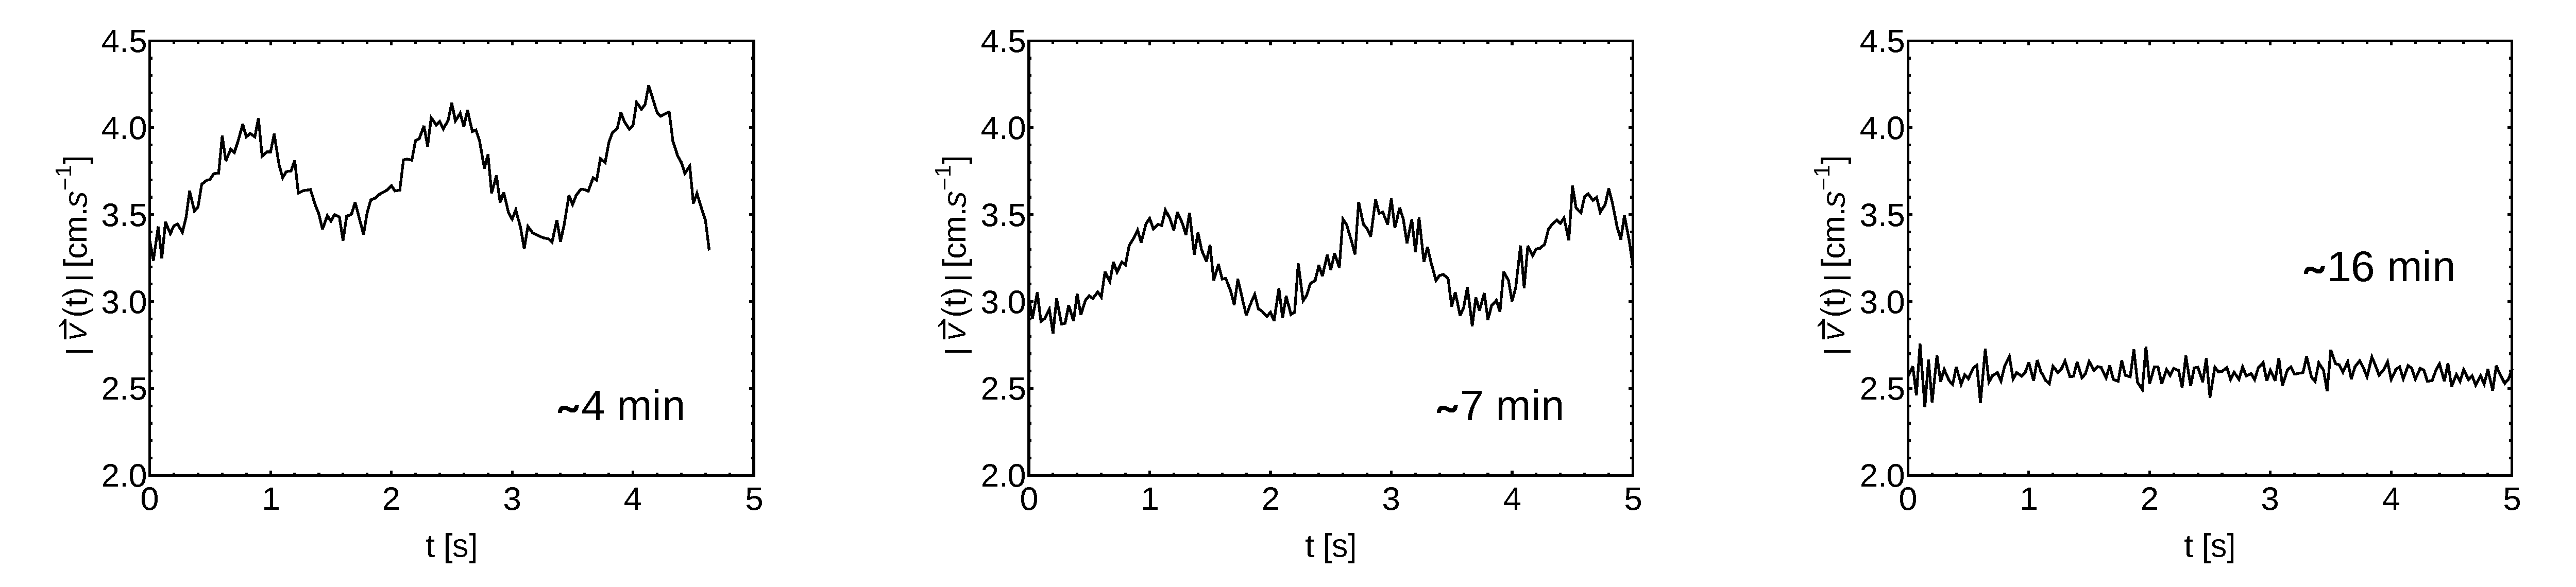
\includegraphics[scale=0.1]{figure7.pdf}
    \end{center}
    \caption{(a) Oscillation in speed of the c-boat at different intervals. (b) The power spectrum of speed.}
    \label{fig:absvnosds}
\end{figure}
The motion of c-boat involves two processes. 1. At an instant position of the c-boat on the air-water interface, Marangoni forces are established because camphoric acid spreads and creates interfacial tension gradients around the c-boat and 2. The Marangoni forces propel the c-boat to a new position where the interfacial tension (concentration of camphoric acid) is high (low). At the new position, the same processes repeat and the c-boat continues to move. Let us define $\tau_{\gamma}$ as the time required to establish sufficient Marangoni forces to overcome the drag forces and $\tau_{\lambda} = \frac{\|\vec{u}\|}{\lambda}$ as the time required for the c-boat to move a distance, $\lambda$ defined as the maximum distance, measured from the center of the c-boat, to which camphoric acid spreads without subliming/evaporating. The c-boat motion can be continous, oscillatory or intermittent when $\tau_{\gamma} < \tau_{\lambda}$, $\tau_{\gamma} \approx \tau_{\lambda}$ or $\tau_{\gamma} > \tau_{\lambda}$ respectively. From the measurements in section~\ref{sec:caspread}, the radius of influence of the c-boat is $\approx 3.6\ \mathrm{cm}$ for a 3 $\mathrm{mm}$ diameter c-boat. Furthermore, the average distance travelled by the c-boat during a period of oscillation ($\approx 1\ \mathrm{Hz}$) is also $\approx$ 3.6 $\mathrm{cm}$. This observation indicates that, the c-boat always moves from one position to another position in steps of $\lambda$ however, the motion appears to be continuous, oscillatory or intermittent depending on $\tau_{\gamma}$ and $\tau_{\lambda}$. A typical c-boat dynamics experiment, with a 3 $\mathrm{mm}$ diameter c-boat, is recorded for 20 minutes during which we observed the oscillatory and continuous motions as shown in figure~\ref{fig:absvnosds}. During the course of the experiment, camphoric acid sublimes into the surroundings resulting in continuous decrease in $\lambda$ of the c-boat, thereby increasing $\tau_{\lambda}$. Therefore, the transistion from $\tau_{\gamma} \approx \tau_{\lambda}$ to $\tau_{\gamma} < \tau_{\lambda}$ leads to oscillatory to continuous motion of the c-boat. Further, to experimentally verify the above hypothesis we used Sodium Dodecyl Sulfate (SDS) to modify the interfacial tension of air-water interface. From equation~\ref{eq:jensen}, modifying the background interfacial tension slows down rate of camphoric acid spread on the air-water interfaction thereby increasing $\tau_{\gamma}$. When the interfacial tension is sufficiently modified, the system goes into $\tau_{\gamma} > \tau_{\lambda}$ regime exhibiting the intermittent motion of the c-boat. Figure~\ref{fig:absvsds} shows the intermittent, oscillatory and continuous regimes at different concentrations of SDS.
\begin{figure}[ht]
    \begin{center}
       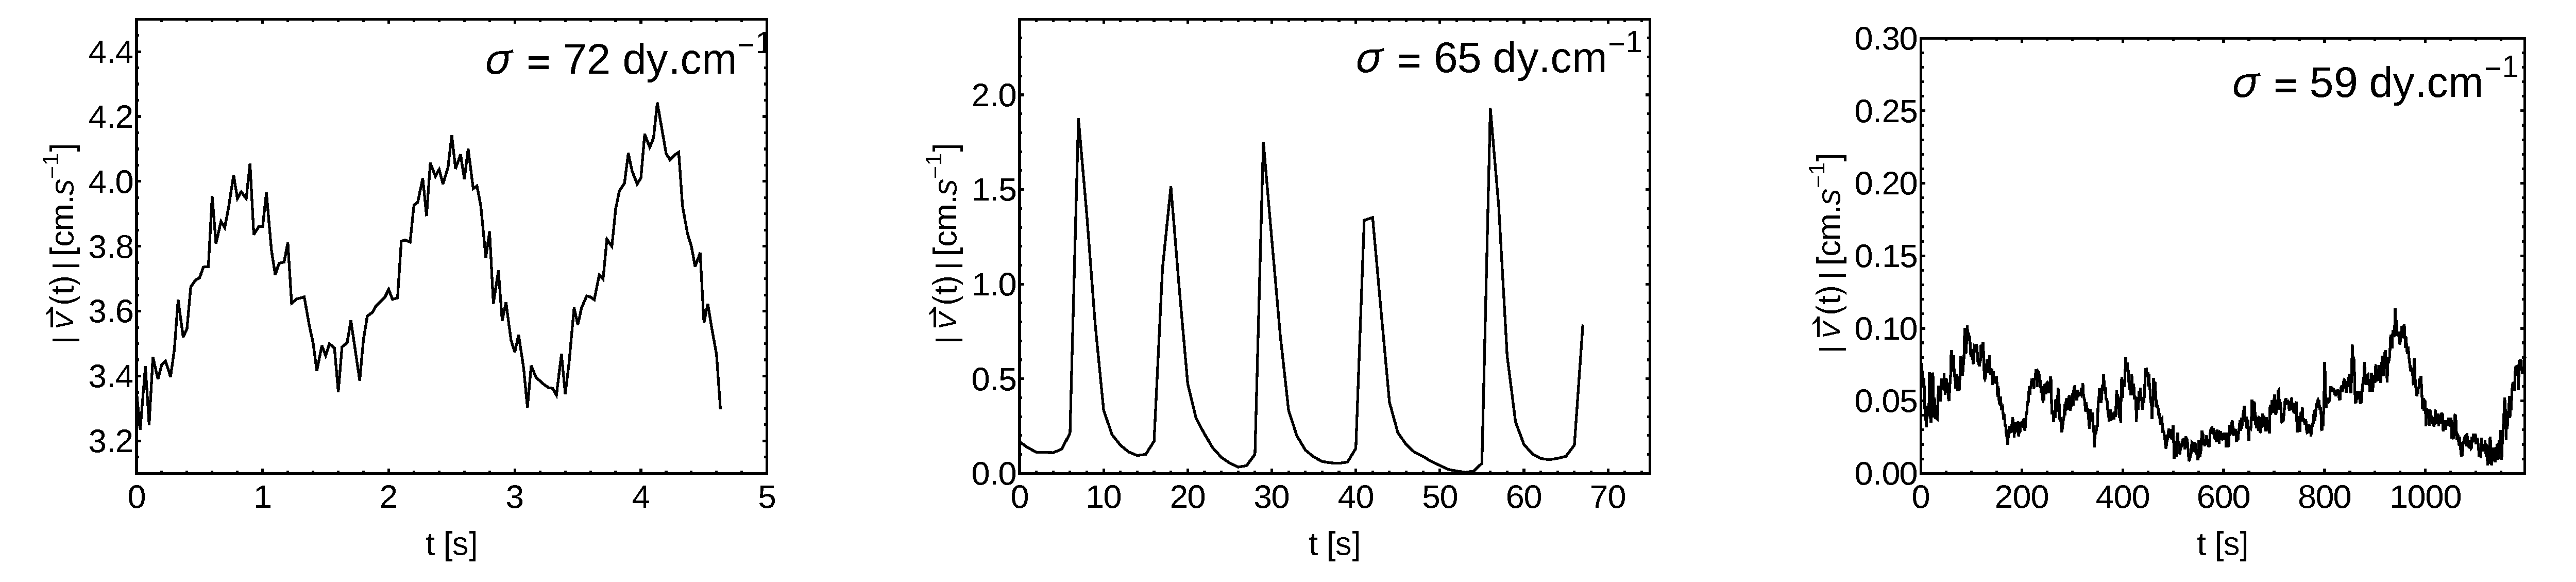
\includegraphics[scale=0.1]{figure8.pdf}
    \end{center}
    \caption{(a) Oscillations in the speed of the c-boat at different concentrations of Sodium Dodecyl Sulfate (SDS) (b) The power spectrum of speed.}
    \label{fig:absvsds}
\end{figure}
\section{Model for Dynamic C-boat}
\begin{align}
\pdc{}{t}c(x, t) &= \mathrm{D} \pdc[2]{}{x}c(x, t) - \tdc{x}{t} \pdc{}{x}c(x, t)  - \xi c(x, t) \\
m\tdc[2]{x}{t} &= -\eta \tdc{x}{t} + \zeta \tdc{}{x}c(x,t) 
\end{align}
\section{Summary}
\label{sec:summary}


\acknowledgments
VSA, DKS, SB and MMB were supported by the OIST Graduate University with subsidy funding from the Cabinet Office, Government of Japan. RKS was hosted by OIST Graduate University on a research internship while performing this work. MMB acknowledges L. Mahadevan for introducing the camphor boat system and subsequent scientific discussions, and D. Vu Anh for help with preliminary experiments.

\bibliography{all}

\end{document} 
